\section{Metodologia}
\label{sec:metodologia}

In questa sezione verranno descritti in dettaglio l'approccio usato per il lavoro di gruppo e le funzioni di reperimento realizzate.


\subsection{Approccio}
\label{sec:approccio}

Il nostro scopo \'e ottenere un valore di Mean Average Precision (\textsc{MAP}) il piu' elevato possibile. Per calcolarla e verificarne il cambiamento durante le varie versioni del codice utilizziamo \texttt{trec\_eval}, esso e' il tool standard usato dalla "TREC community" per valutare un'esecuzione ad hoc, dandole il file contenete i risultati e un set standard di risultati giudicati.  

Abbiamo optato approccio probabilistico con \texttt{Okapi BM25} per la risoluzione dei laboratori, poiche' \'e un buon modello ed \'e stato usato con successo da esperti nel campo.  
Abbiamo utilizzato il linguaggio Python per implementare il codice, utilizzando diverse librerie contenenti metodi, a noi, utili: \texttt{numpy} gestione delle matrici, \texttt{matplotlib} gestione dei plot (grafici), \texttt{networkx} gestione dei grafi.
Oltre a \texttt{Python} abbiamo utilizzato altri software per il lavoro: \texttt{Git}, \'e un sistema di versionamento distribuito, per lo scambio del codice e l'aggiornamento delle diverse versioni di quest'ultimo e \texttt{latex} per la scrittura dei pdf di report.
Per ogni esercitazioni \'e stato utilizzato un approccio di gruppo, attraverso discussioni sull'implementazione e sui risultati durante il laboratorio.

\subsection{Indicizzazione} \label{sec:metodi-di-indic}

\paragraph{\textbf{Descrizione.}} Costruzione di un algoritmo di indicizzazione in grado di costruire delle strutture dati necessarie al reperimento tramite \textsc{bm25}. 

\paragraph{\textbf{Implementazione.}}
Per l'implementazione e' stato utilizzato il file \textit{freq.docid.stem.txt} che contiene le frequenze delle keywords (dopo lo stemming) nei documenti. Poiche' le stop words sono gia' state rimosse da tale file, ignoriamo la stoplist.
L'algoritmo di indicizzazione utilizza le keywords presenti in tale file per costruire un dizionario delle keywords presenti nella collezione. In seguito scorre sulle righe del file \textit{freq.docid.stem.txt} e costruisce la Document Term Matrix (DTM), una matrice di  dimensione $n_{docs} \times n_{words}$ che contiene in posizione $(i,j)$ il numero di occorrenze del termine $j$ nel documento $i$. Infine salva su file le seguenti strutture:
\begin{itemize}
	\item Le lunghezze (numero di termini) dei documenti, necessarie alla normalizzazione sulla lunghezza in \textsc{bm25},
	\item La DTM normalizzata sui colonne, cioe' una matrice delle frequenze che contiene in posizione $(i,j)$ la frequenza del termine $j$ nel documento $i$,
	\item Il dizionario contenente le keywords della collezione.
\end{itemize}

\subsection{Reperimento}
\label{sec:metodi-di-reper}

\paragraph{\textbf{Descrizione}}: comprensione dei meccanismi di reperimento e costruzione di un primo algoritmo di reperimento.
Implementeremo l'algoritmo \textsc{BM25}, che presa in input una query restituira' una lista ordinata di documenti con i relativi $score_{bm25}$.

\paragraph{\textbf{Implementazione}}: 
Per effettuare l'implementazione useremo le tre strutture ottenute dall'indicizzazione e un dizionario che contiene le parole stemmate per ogni query creato utilizzando il file \textit{query-stem.txt}. Per ogni query $Q$, l'algoritmo effettuera' il retrieval scorrendo la lista degli stem $qw$ della query e per ogniuna di esse interroga il dizionario per ottenere l'indice della posizione occupata nella matrice delle frequenze. Cosi' facendo \'e in grado di ottenere le frequenze di ogni parola per ogni documento e calcolare lo score di quest'ultimo, infine ordina in modo decrescente i documenti aventi punteggi maggiori di zero.
\begin{algorithmic}
\State $Q \gets query$
\State $D \gets dictionary$
\State $C \gets documents$
\State $F \gets frequency matrix$
\ForAll{$qw \in Q$}
	\State $index\_of\_words \gets extract(D,qw)$
	\ForAll{$doc \in C$}
		\ForAll{$id \in index\_of\_words$}
			\State $f_{bm25} \gets extract\_frequency(F,doc,id)$
		\EndFor
		\State $score_{bm25} \gets score_{bm25} + f_{bm25}$
	\EndFor
\EndFor\\
\Return top $k$ scoring documents
\end{algorithmic}
Tale algoritmo ha complessita' $O(n \cdot m)$, dove $n$ e' il numero di documenti nella collezione ed $m$ e' il numero di descrittori nell'interrogazione (query) $Q$, dallo pseudo codice tale complessita' non \'e chiara ma nell'implementazione di tale algoritmo la ricerca degli $id$ \'e stata fatta utilizzando delle funzioni proprie di Python il che' le rende ininfluenti sul calcolo della complessita'. 

\subsection{Relevance Feedback}
\label{sec:relevance-feedback}

\paragraph{\textbf{Descrizione}}: comprensione del Relevance Feedback (\textsc{RF}) e scrittura di una funzione di reperimento equipaggiata con \textsc{RF esplicito} e una seconda con \textsc{RF pseudo}.
Durante il calcolo di \textsc{BM25} terremo conto dei giudizi di rilevanza.
BM25:
\[ \sum\limits_{i \in Q}\log\Bigl(\frac{(r_i+0.5)/(R-r_i+0.5)}{(n_i-r_i+0.5)/(N-n_i-R+r_i+0.5)}\Bigl)\cdot\frac{(k_1+1)f_i}{k+f_i}\cdot\frac{(k_2+1)qf_i}{k_2+qf_i}. \]
La formula di BM25 tiene gia' in considerazione i giudizi di rilevanza, infatti $R$ rappresenta il numero di documenti rilevanti per la query presa in considerazione, mentre il valore di $r_i$ rappresenta il numero di documenti rilevanti che contengono il termine $i$, quindi costruiremo un algoritmo in grado di calcolarli.

\paragraph{\textbf{Implementazione}}: 
L'implementazione dei due algoritmo \'e differente, poiche' il calcolo dello \textsc{Pseudo RF} richiede due passi, mentre ne basta uno solo per \textit{RF Esplicito}.
\begin{itemize}
\item \textsc{RF Esplicito}: verra' utilizzato il file \textit{qrels-treceval.txt} per estrarre i valori di $R$ ed $r_i$, i quali saranno utilizzati all'interno del calcolo di bm25.
\item \textsc{Pseudo RF}: il primo passo consiste nel caclolo del ranking senza informazioni di rilevanza, verranno poi considerati rilevanti i primi $N$ documenti, con tali documenti verranno trovati i valori di $R$ ed $r_i$ utilizzati per la seconda esecuzione dell'algoritmo.
\end{itemize}
Per poter effettuare il calcolo dei valori di $R$ ed $r_i$ l'algoritmo utilizzera' la matrice che contiene le frequenze delle perole di ogni documento (sezione 2.2). Durante il reperimento per ogni documento e per ogni termine $i$ l'algoritmo calcola il numero di documenti considerati rilevanti che lo contengono e salvera' tale valore in una mappa $map$ (mappa $i$->$r_i$), con questa mappa l'algoritmo calcola il ranking rispetto ai valori di $R$ ed $r_i$.



\subsection{PageRank}
\label{sec:pagerank}

\paragraph{\textbf{Descrizione}}: comprensione di PageRank, implementazione di PageRank e scrittura di una funzione di reperimento che lo integri.
la funzione di reperimento combinera' gli score di BM25 ($rk$) con il valore del pagerank ($pr$) attraverso la seguente formula:
\[ score =  \alpha \cdot rk + (1-\alpha) \cdot pr,\]
dove $\alpha$ e' un parametro che varia tra 0 ed 1 e, quindi, sposta il peso uniformemente da pagerank a BM25.
Ma poter effettuare questo confronto in modo coerente, entrambe le distribuzioni devono essere ridimensionate, si effettua quindi una normalizzazione in modo da avere valori compresi tra 0 e 1. Per far cio' abbiamo usato la formula:
\[ z_i = \frac{x_i - min(x)}{max(x) - min(x)}, \]


\paragraph{\textbf{Implementazione}}: per effettuare il calcolo del pagerank abbiamo utilizzato la libreria \texttt{networkx}, essa attraverso il metodo \texttt{read\_edgelist} permette la costruzione del grafo delle citazioni a partire dalla lista di archi. Inoltre dispone del metodo \texttt{pagerank} per la computazione del pagerank utilizzando \texttt{power iteration} sulla matrice di transizione, tale computazione e' fatta a tempo di indexing e i valori verranno utilizzati a tempo di retrieval.

\subsection{Latent Semantic Analysis}
\label{sec:lsa}

\paragraph{\textbf{Descrizione}}: comprensione di Latent Semantic Analysis (LSA), implementazione di LSA e costruzione di una funzione di reperimento che implementi LSA.
Come funzione di ranking sara' usata la BM25 con relevance feedback esplicito (laboratorio 5) e verra' applicata LSA. 


\paragraph{\textbf{Implementazione}}: l'algoritmo calcolera' quindi la BM25 con relevance feedback esplicito e prendera' in considerazione soltanto i primi $N$ documenti reperiti. Utilizzera' il metodo \texttt{linalg.svd} (appartenente alla libreria \texttt{numpy}) per il calcolo della fattorizzazione della matrice termini-documenti $X$: 
\[ X = U \Sigma V^{T}. \]\\
Da questa matrice derivera' la matrice ridotta tenendo in considerazione soltanto $m$ dimensioni. Di seguito effettuera' la proiezione di $\vec{q}$ sullo spazio a dimensione ridotto secondo la formula: 
\[ \vec{q}_m = \Sigma^{-1}_m U^{T}_m \vec{q}. \]
Infine computera' la \textit{cosine similarity} tra le rappresentazione degli $N$ documenti nello spazio ridotto (cioe' le colonne $V^{T}$) e la query ridotta $\vec{q}$, riordinera' i risultati di questi $N$ documenti in ordini decrescente e ad essi verranno accodati i restanti documenti calcolati ad inizio algoritmo tramite BM25 con relevance feedback esplicito.


\subsection{Hyper-linked Induced Topic Search}
\label{sec:hits}

\paragraph{\textbf{Descrizione}}: comprensione di Hyperlinked Induced Topic Search (\textsc{HITS}), implementazione e costruzione di una funzione di reperimento che implementi \textsc{HITS}.

\paragraph{\textbf{Implementazione}}: l'algoritmo da noi scritto effettua il ranking tramite la funzione BM25 (laboratorio 3 - sezione \ref{sec:metodi-di-reper}), utilizzando i primi $N$ documenti costruisce il corrispondente grafo delle citazioni $R_q$. Quest'ultimo viene espanso per ottenere un grafo allargato $B_q$ sul quale calcolare \textsc{HITS}.
In figura \ref{fig:unodue} \'e rappresentata la relazione tra il grafo radice $R_q$ e il grafo allargato $B_q$ per capirne le dinamiche di espansione (i grafi si riferiscono alla query $56$).
\begin{figure}
	\centering
	\begin{subfigure}{.5\textwidth}
		\centering
		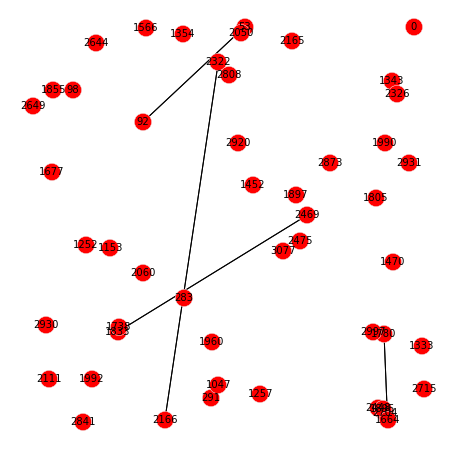
\includegraphics[width=1\textwidth]{figures/R.png}
		\caption{Grafo radice ($R_{56}$)}
		\label{fig:uno}
	\end{subfigure}%
	\begin{subfigure}{.5\textwidth}
		\centering
		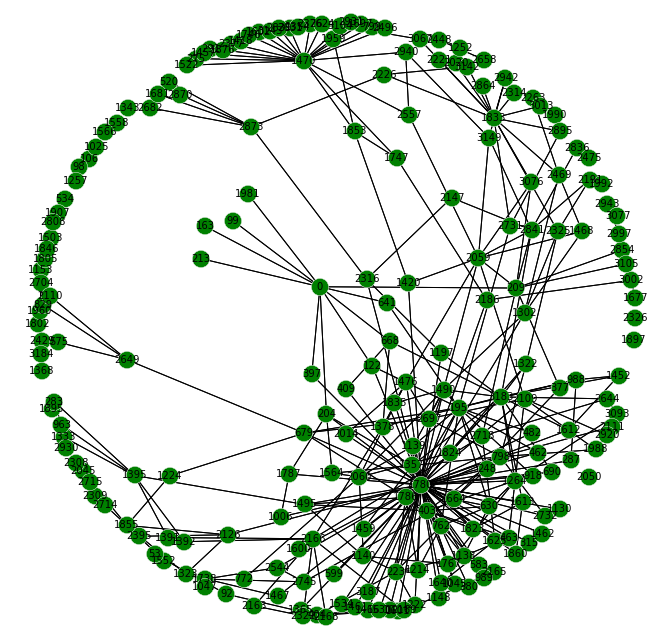
\includegraphics[width=1\textwidth]{figures/B.png}
		\caption{Grafo base ($B_{56}$).}
		\label{fig:due}
	\end{subfigure}
	\caption{Grafi ottenuti applicando \textsc{HITS} sui top $N=50$ documenti per la query $56$.}
	\label{fig:unodue}
\end{figure}

Abbiamo poi combinato, per i primi $N$ documenti, gli score di BM25 (\textit{sc}) con i punteggi di authority (\texttt{auth}) e hubbiness (\texttt{hub}) attraverso la formula:
\[ hits_{score} =  \alpha \cdot sc + \beta \cdot auth + \gamma \cdot hub,\]
Il valore del parametro $\alpha$ varia in [0, 1],  mentre quello di $\beta$ e $\gamma$ puo' variare tra [-1, 1], in quanto si vogliono cogliere possibili influenze negative. I valori di $sc, auth, hub$ vengono normalizzati nell'intervallo [0, 1] prima del calcolo. 
Infine l'algoritmo riordina i documenti reperiti per valori decrescenti di $hits_{score}$.


\subsection{Evolution Strategy}
\label{sec:es}

Per ottimizzare gli algoritmi di reperimento abbiamo scelto di utilizzare un Evolution Strategy~\cite{back1996evolutionary} (ES) che e' una tecnica di ottimizzazione basata sui principi che regolano l'evoluzione. Tecniche di questo tipo sono piu' robuste rispetto ai metodi di ricerca lineare per quanto riguardo i massimi locali. Il loro svantaggio consiste nel maggior numero di valutazioni richieste. Nel nostro contesto una valutazione impiega circa 3-15 secondi a seconda della complessita' del metodo di reperimento. Cio' permette di eseguire l'algoritmo di ottimizzazione in un tempo accettabile.

I parametri che abbiamo scelto di ottimizzare cambiano in base alla funzione di reperimento (e quindi del laboratorio). Per il laboratorio 3, 4, 6 abbiamo scelto di ottimizzare $k_1, b$. Ignoriamo $k_2$ in quando abbiamo visto che non ci sono termini ripetuti nelle query e quindi tale termine non influisce sul punteggio. Per il laboratorio 5 ottimizziamo $k_1, b, \alpha$. Per il laboratorio 7 ottimizziamo $k_1, b, \alpha, \beta, \gamma$. Per lo pseudo relevance feedback del laboratorio 4 il numero di documenti considerati rilevanti $R = 50$, mentre per l'\textsc{lsa} del laboratorio 6 il numero di documenti da riordinare $N = 30$, e il numero di dimensioni per la riduzione $m=2$ (tali parametri sono interi e non si prestano ad un'ottimizzazione tramite ES). La funzione da massimizzare \'e la Mean Average Precision.

Figura \ref{fig:es_all} riporta l'andamento della MAP durante l'ottimizzazione della funzione di reperimento dei laboratori. 
\begin{figure*}
        \centering
        \begin{subfigure}[htpb]{0.475\textwidth}
            \centering
            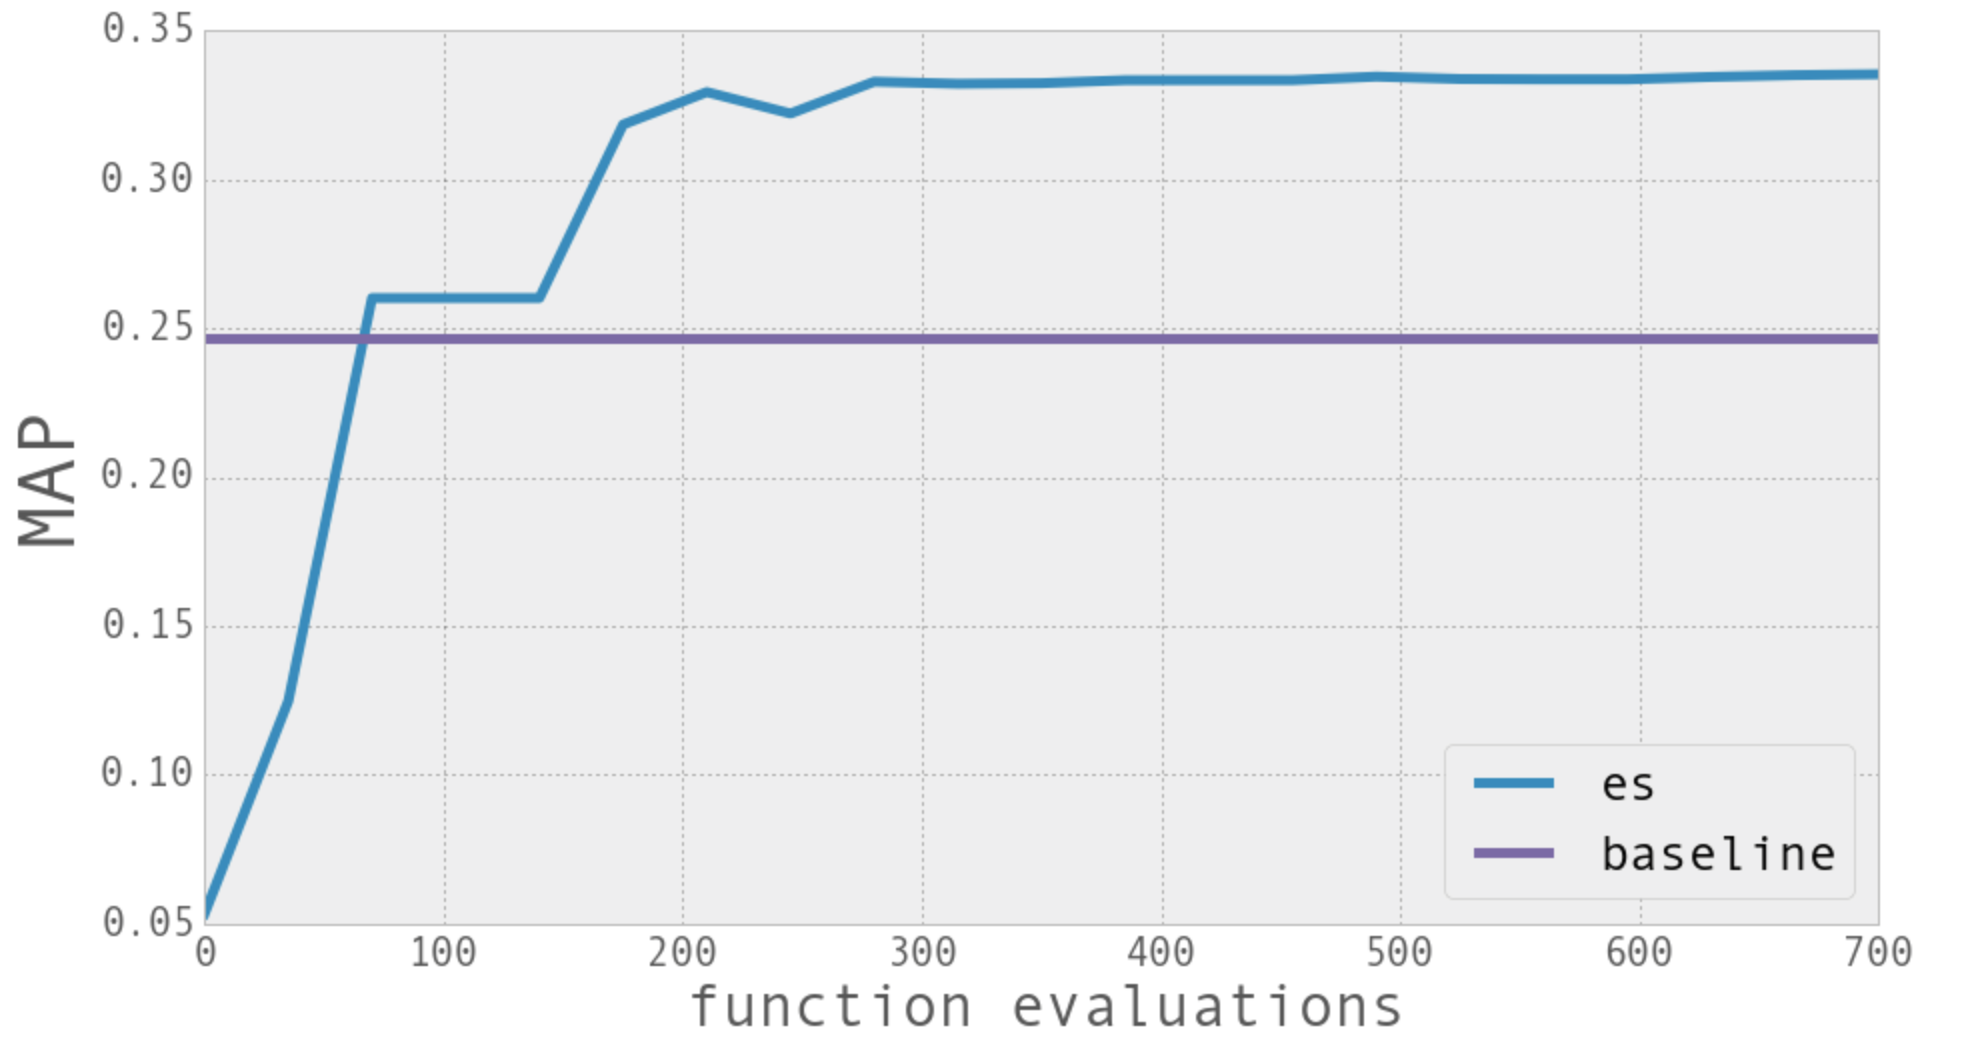
\includegraphics[width=\textwidth]{figures/es_lab3.png}
            \caption[Network2]%
            {{\small Laboratorio 3 (\textsc{baseline})}}    
            \label{fig:es_lab3}
        \end{subfigure}
        \hfill
        \begin{subfigure}[htpb]{0.475\textwidth}  
            \centering 
            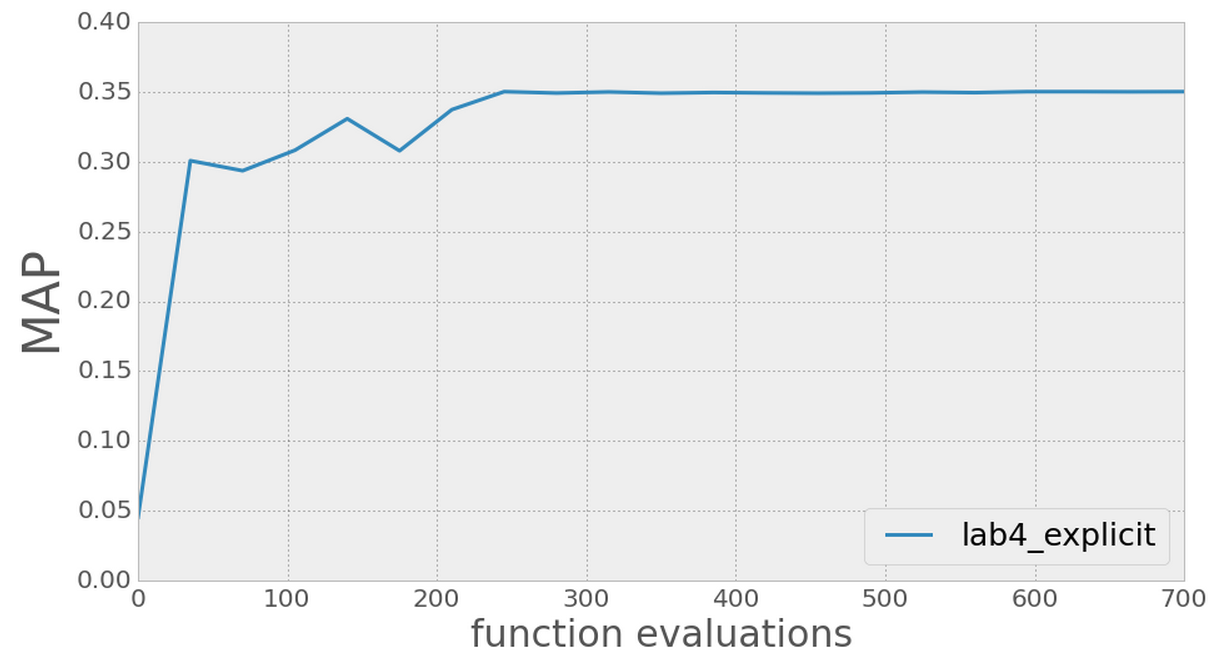
\includegraphics[width=\textwidth]{figures/es_lab4_e.png}
            \caption[]%
            {{\small Laboratorio 4 (\textsc{rf} esplicito)}}    
            \label{fig:es_lab4_esp}
        \end{subfigure}
        \vskip\baselineskip
        \begin{subfigure}[htpb]{0.475\textwidth}   
            \centering 
            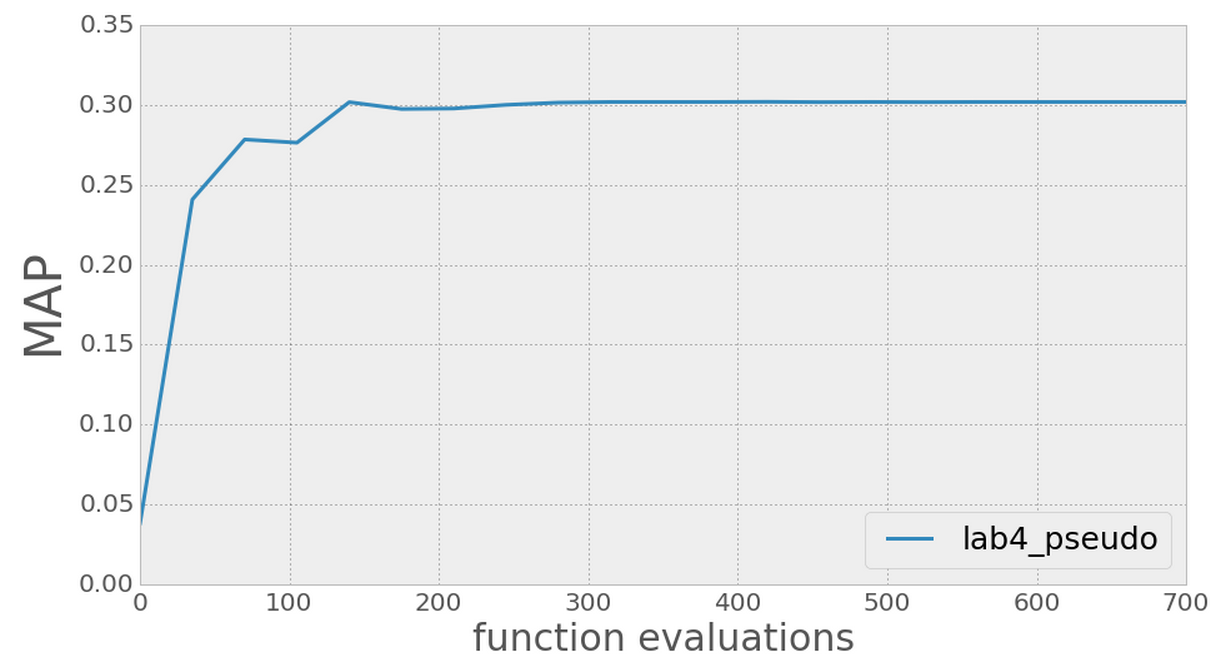
\includegraphics[width=\textwidth]{figures/es_lab4_p.png}
            \caption[]%
            {{\small Laboratorio 4 (\textsc{rf} pseudo)}}    
            \label{fig:es_lab4_pse}
        \end{subfigure}
        \quad
        \begin{subfigure}[htpb]{0.475\textwidth}   
            \centering 
            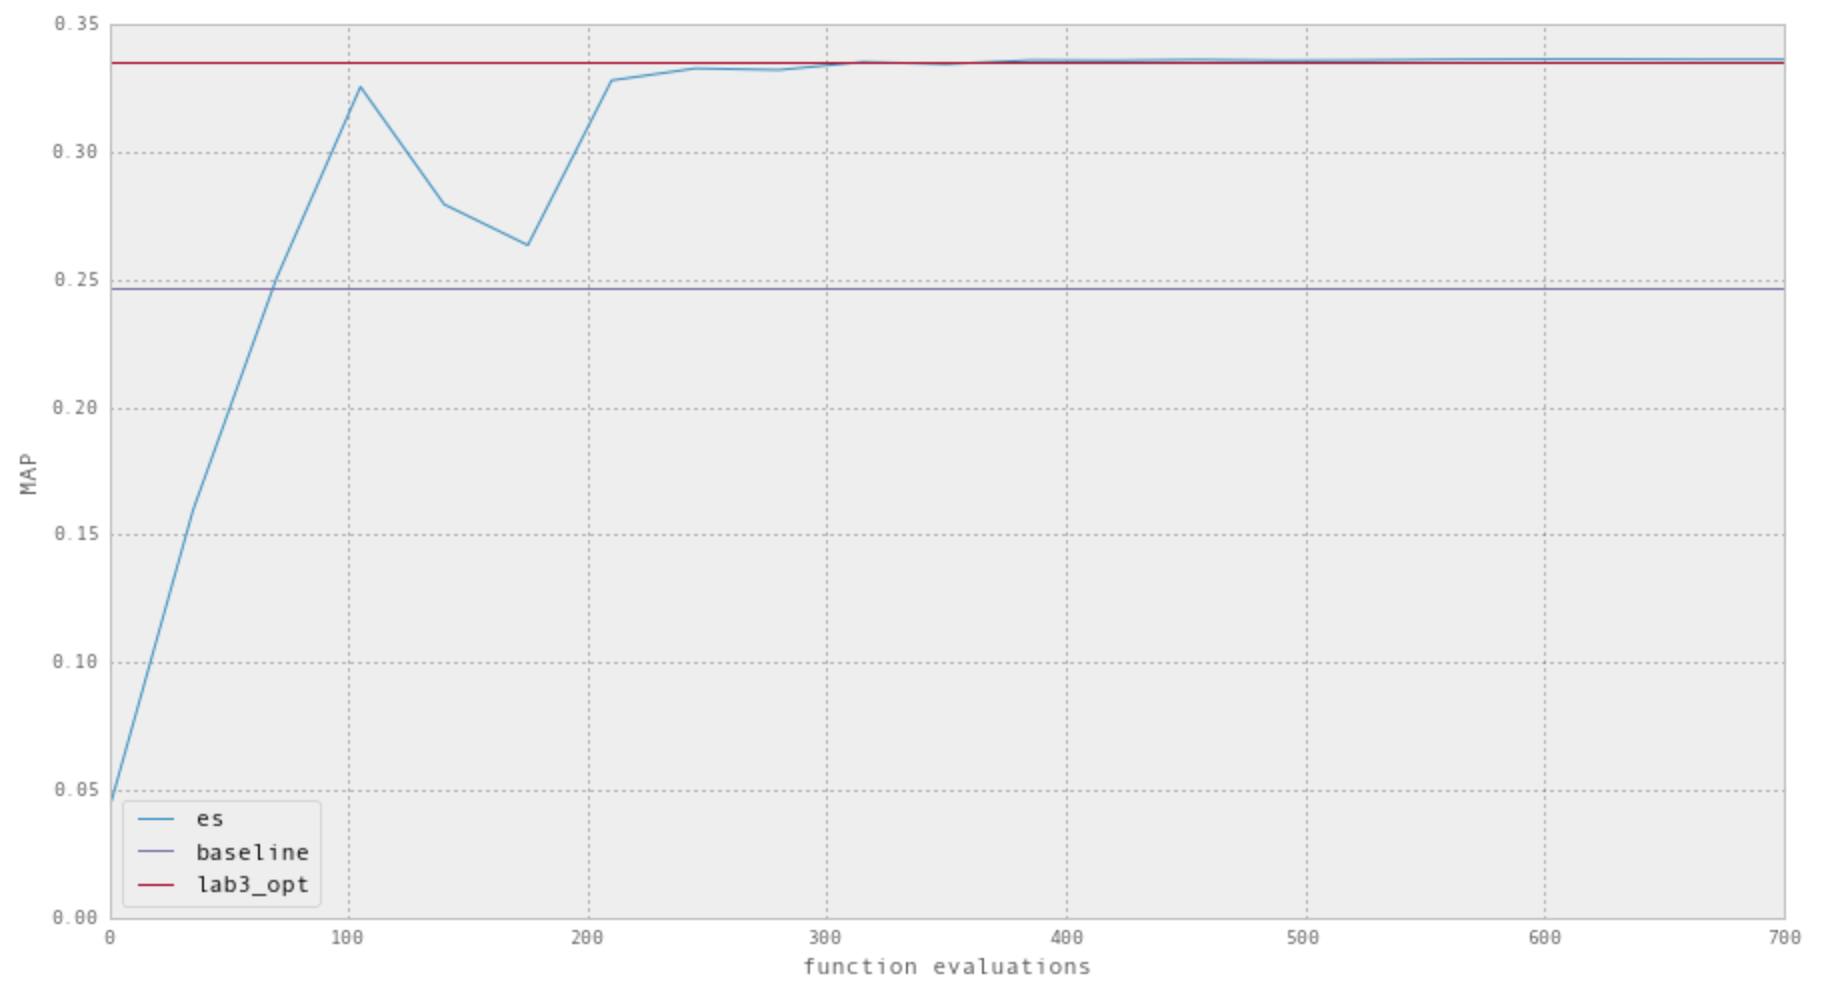
\includegraphics[width=\textwidth]{figures/es_lab5.png}
            \caption[]%
            {{\small Laboratorio 5 (\textsc{pagerank})}}    
            \label{fig:es_lab5_esp}
        \end{subfigure}
        \vskip\baselineskip
        \begin{subfigure}[htpb]{0.475\textwidth}  
            \centering 
            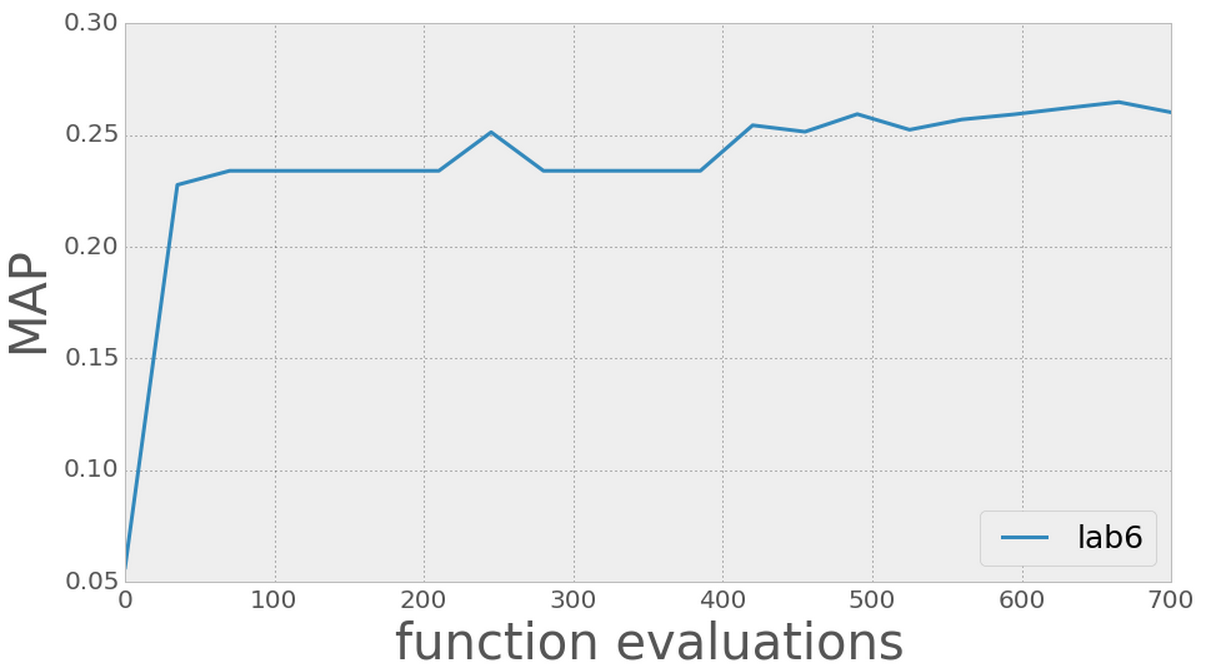
\includegraphics[width=\textwidth]{figures/es_lab6.png}
            \caption[]%
            {{\small Laboratorio 6 (\textsc{lsa})}}    
            \label{fig:es_lab6}
        \end{subfigure}
        \quad
        \begin{subfigure}[htpb]{0.475\textwidth}   
            \centering 
            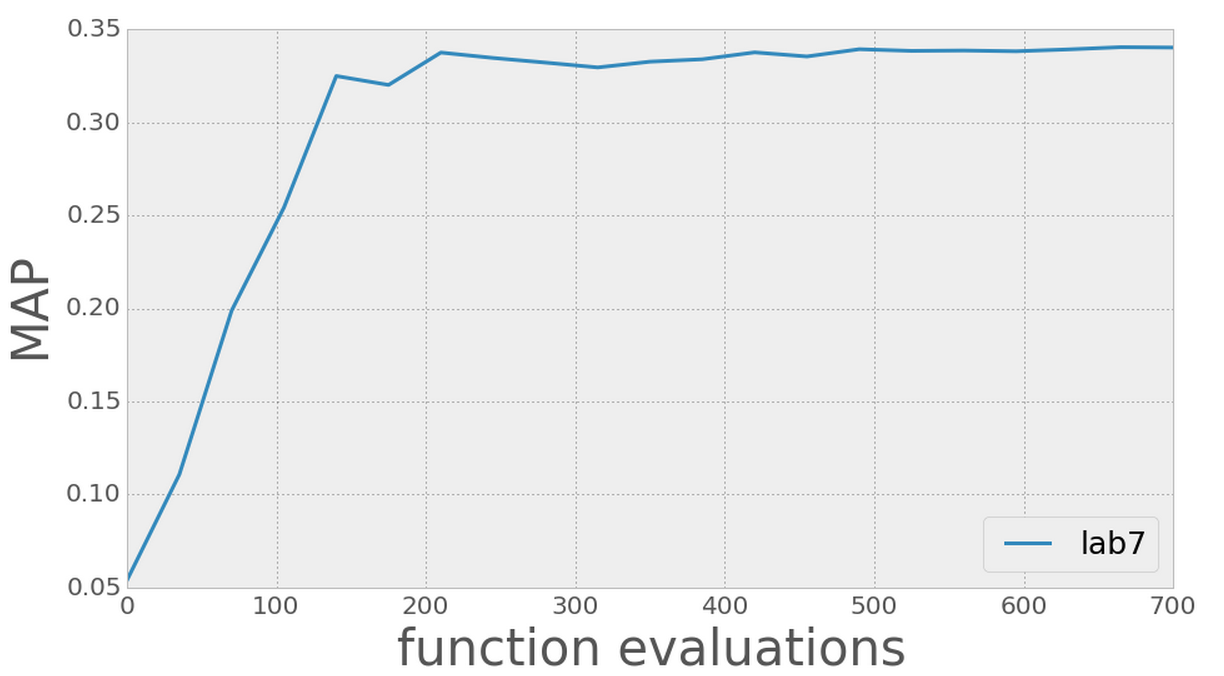
\includegraphics[width=\textwidth]{figures/es_lab7.png}
            \caption[]%
            {{\small Laboratorio 7 (\textsc{hits})}}    
            \label{fig:es_lab7}
        \end{subfigure}
        \caption[ The average and standard deviation of critical parameters ]
        {\small Valore MAP durante iterazioni dell'ES, per le funzioni di reperimento dei vari laboratori.} 
        \label{fig:es_all}
\end{figure*}
Tabella \ref{tab:es} riporta i risultati dell'ottimizzazione.
\begin{table}[htpb]

\begin{center}
\begin{tabular}{|c|c|c|}
\hline
metodo & parametri ottimizzati & MAP \\
 \hline
\textsc{baseline} & $k_1 = 0.0253, b = 0.0221$ & $0.3354$ \\
\textsc{rf} esplicito & $k_1 = 0.02065, b = 0.0$ & $0.3504$ \\
\textsc{rf} pseudo & $k_1 = 0.02065, b = 0.0$ & $0.3022$ \\
\textsc{pagerank} & $k_1 = 0.0237, b = 0.0, \alpha=0.7832$ & $0.3366$ \\
\textsc{lsa} & $k_1 = 0.0087, b = 0.0$ & $0.2648$ \\
\textsc{hits} & $k_1 = 0.0247, b = 0.0185, \alpha=1.0, \beta=0.1098, \gamma=0.0549$ & $0.3405$ \\
\hline
\end{tabular}
\end{center}
\caption{Risultati ottimizzazione con ES per le funzioni di reperimento dei vari laboratori.}
\label{tab:es}
\end{table}

Grazie all'ES si \'e ottenuto un notevole miglioramento rispetto alla prima versione dove i parametri sono stati scelti empiricamente, e il valore di MAP si aggirava attorno al $0.25$. Inoltre dai grafici si puo' notare come l'algoritmo di ottimizzazione sia molto robusto, dato che dopo $\sim{300}$ valutazioni \'e gia' molto vicino alla configurazione ottima. I risultati dell'ottimizzazione vengono discussi in Sezione \ref{sec:risult-sper}.

\subsection{Altri metodi}
tipo lucene
\label{sec:altri-metodi}

Se sono stati sviluppati altri metodi, descriverli qui.

